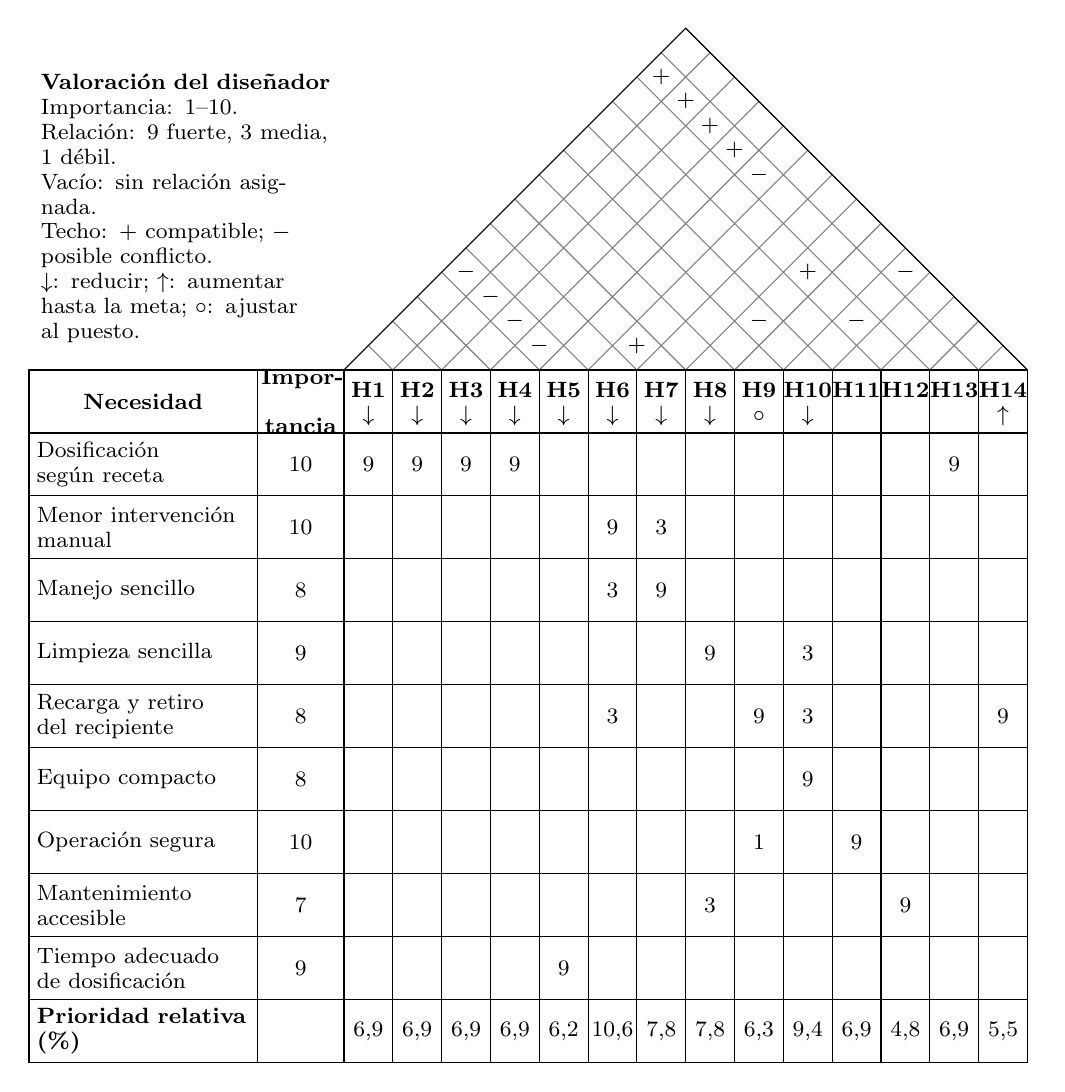
\begin{tikzpicture}[font=\fontsize{8}{9}\selectfont]
    % Catorce características; el techo muestra hipótesis de interacción.
    \begin{scope}
        \clip (0,0) -- (8.68,0) -- (4.34,4.34) -- cycle;
        \foreach \k in {0,...,14} {
            \draw[gray] (\k*0.62,0) -- ++(4.34,4.34);
            \draw[gray] (\k*0.62,0) -- ++(-4.34,4.34);
        }
    \end{scope}
    \draw (0,0) -- (4.34,4.34) -- (8.68,0);
    \foreach \i/\j/\s in {
        1/5/-,2/5/-,3/5/-,4/5/-,5/13/-,6/7/+,
        8/10/-,8/12/+,10/12/-,10/14/-,
        1/13/+,2/13/+,3/13/+,4/13/+} {
        \node at ({0.62*((\i+\j)/2-0.5)},{0.31*(\j-\i)}) {$\s$};
    }
    \node[align=left,text width=37mm,anchor=center] at (-2,2.05)
        {\textbf{Valoración del diseñador}\\
        Importancia: 1--10.\\
        Relación: 9 fuerte, 3 media, 1 débil.\\
        Vacío: sin relación asignada.\\
        Techo: $+$ compatible; $-$ posible conflicto.\\
        $\downarrow$: reducir; $\uparrow$: aumentar hasta la meta; $\circ$: ajustar al puesto.};
    \draw (-4,0) rectangle (8.68,-8.8);
    \draw (-1.1,0) -- (-1.1,-8.8);
    \draw (0,0) -- (0,-8.8);
    \foreach \k in {1,...,13} {\draw (\k*0.62,0) -- (\k*0.62,-8.8);}
    \foreach \k in {1,...,10} {\draw (-4,-\k*0.8) -- (8.68,-\k*0.8);}
    \node[align=center,text width=27mm] at (-2.55,-0.4) {\textbf{Necesidad}};
    \node[align=center,text width=10mm] at (-0.55,-0.4) {\textbf{Impor-}\\\textbf{tancia}};
    \foreach \k in {1,...,14} {\node at ({(\k-0.5)*0.62},-0.25) {\textbf{H\k}};}
    \foreach \k in {1,...,8,10,...,13} {\node at ({(\k-0.5)*0.62},-0.59) {$\downarrow$};}
    \node at ({(9-0.5)*0.62},-0.59) {$\circ$};
    \node at ({(14-0.5)*0.62},-0.59) {$\uparrow$};
    \foreach \r/\texto/\peso in {
        1/{Dosificación\\según receta}/10,
        2/{Menor intervención\\manual}/10,
        3/{Manejo sencillo}/8,
        4/{Limpieza sencilla}/9,
        5/{Recarga y retiro\\del recipiente}/8,
        6/{Equipo compacto}/8,
        7/{Operación segura}/10,
        8/{Mantenimiento\\accesible}/7,
        9/{Tiempo adecuado\\de dosificación}/9} {
        \node[align=left,text width=27mm] at (-2.55,{-0.4-0.8*\r}) {\texto};
        \node at (-0.55,{-0.4-0.8*\r}) {\peso};
    }
    \foreach \r/\c/\v in {
        1/1/9,1/2/9,1/3/9,1/4/9,1/13/9,
        2/6/9,2/7/3,3/6/3,3/7/9,4/8/9,4/10/3,
        5/6/3,5/9/9,5/10/3,5/14/9,6/10/9,
        7/9/1,7/11/9,8/8/3,8/12/9,9/5/9} {
        \node at ({(\c-0.5)*0.62},{-0.4-0.8*\r}) {\v};
    }
    \node[align=left,text width=27mm] at (-2.55,-8.4) {\textbf{Prioridad relativa (\%)}};
    \foreach \c/\p in {1/{6,9},2/{6,9},3/{6,9},4/{6,9},5/{6,2},6/{10,6},7/{7,8},8/{7,8},9/{6,3},10/{9,4},11/{6,9},12/{4,8},13/{6,9},14/{5,5}} {
        \node at ({(\c-0.5)*0.62},-8.4) {\p};
    }
\end{tikzpicture}
